\documentclass[12pt]{article}
\usepackage[a4paper, total={6in, 9in}]{geometry}
\usepackage{graphicx}
\graphicspath{ {./images/output/} }
\usepackage{caption}
\usepackage[english]{babel}
\usepackage{titling}
\usepackage{float}
\usepackage{amsmath}
\usepackage{minted}
% \usepackage{multicol}
% \usepackage{array}
% \usepackage{setspace}
% \usepackage{placeins}
\usepackage{parskip}

% \usepackage{lipsum}

\title{ Implementation of NMOS Ratio-less Inverter}
\author{}
\date{}

\pagenumbering{gobble}
\begin{document}
\vspace*{\fill}
\begin{center}

    \emph{Heaven's Light is Our Guide} \\
    \textbf{Rajshahi University of Engineering and Technology} \\

    \begin{figure}[H]
        \centering
        
\includegraphics[scale=.34]{images/RUET_logo.png}
        \label{fig:ruet_logo}
    \end{figure}
    \vspace{5mm}

    \textbf{Course Code}\\
    ECE 4128\\
    \vspace{3mm}
    \textbf{Course Title}\\
    VLSI Design

    \vspace{5mm}
    \textbf{Experiment Date:} {July 4, 2025},\\
    \textbf{Submission Date:} {August 11, 2025}\\

    \vspace{5mm}
    \textbf{Lab Report 2: \\
        Implementation of NMOS Ratio-less Inverter.}

    \vspace{15mm}

    \begin{tabular}{c|c}
        \textbf{Submitted to} & \textbf{Submitted by} \\
        Moloy Kumar Ghosh     &                       \\
        Lecturer              &                       \\
        Dept of ECE, RUET     & Md. Tajim An Noor     \\
        \&                    & Roll: 2010025         \\
        Md. Faysal Ahamed     &                       \\
        Lecturer              &                       \\
        Dept of ECE, RUET     &                       \\
    \end{tabular}

\end{center}
\vspace*{\fill}


\pagebreak

\tableofcontents

\pagebreak
\pagenumbering{arabic}
\maketitle

\section*{Theory}
\addcontentsline{toc}{section}{Theory}
An inverter is a fundamental digital logic gate that outputs the logical opposite of its input~\cite{weste2015cmos}. In transistor-based designs, inverters can be constructed using CMOS technology, which combines PMOS and NMOS transistors, or using NMOS-only approaches~\cite{kang2003cmos}. In NMOS logic, both the pull-up and pull-down networks utilize NMOS transistors. Traditionally, a load resistor connects the supply voltage (VDD) to the output node, while an NMOS transistor pulls the output to ground. However, physical resistors are inefficient in terms of area and speed for integrated circuits, especially as circuit complexity increases~\cite{sze2008physics}.

To address these limitations, active load NMOS transistors can replace the resistor, resulting in a ratio-less inverter design~\cite{rabaey2003digital}. This configuration, known as the 3-NMOS ratio-less inverter, uses three NMOS transistors: one as the main driver and two as active loads. The driver transistor receives the input signal at its gate and connects its source to ground. The active load transistors are placed between VDD and the output node, with their gates biased to remain partially on, acting as constant current sources. This approach simplifies fabrication in NMOS technology and eliminates the need for precise transistor sizing ratios, making it suitable for large-scale integration~\cite{kang2003cmos}.

\begin{figure}[H]
    \centering
    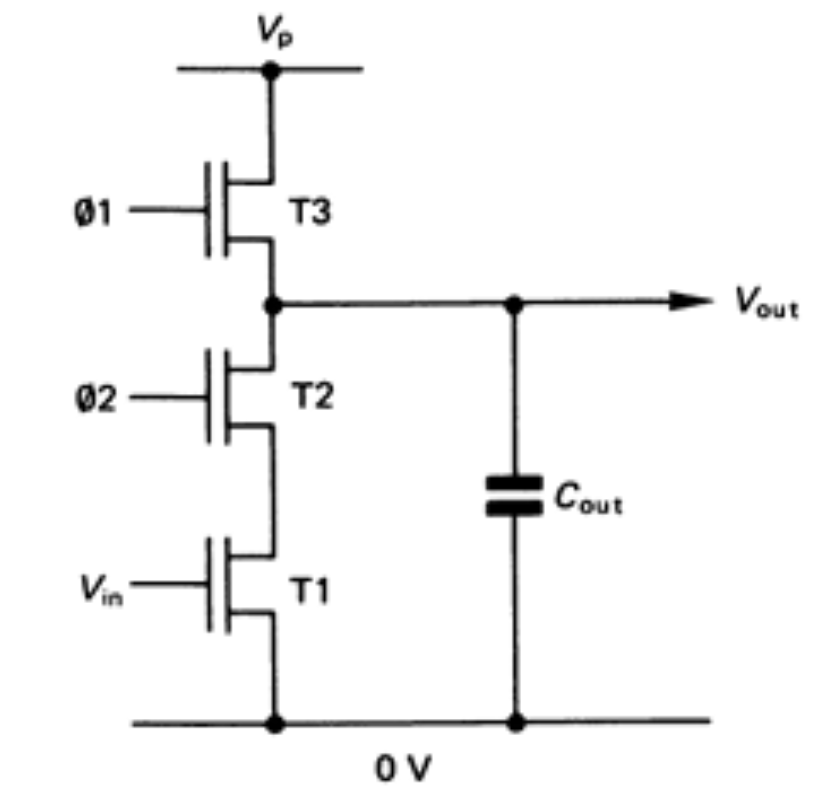
\includegraphics[width=0.4\textwidth]{th.png}
    \caption{Schematic diagram of the NMOS ratio-less inverter}
\end{figure}

\subsection*{Operation}
\addcontentsline{toc}{subsection}{Operation}
\begin{enumerate}
    \item \textbf{Input Low (Logic 0):} When the input is at logic 0, transistor T1 remains OFF. The active load transistors (T2 and T3) conduct sufficient current to raise the output voltage to logic 1.
    \item \textbf{Input High (Logic 1):} When the input switches to logic 1, T1 turns ON, creating a low-resistance path from the output node to ground. This pulls the output down to logic 0. The active load transistors continue to conduct a small amount of current, resulting in static power consumption.
\end{enumerate}

\section*{Required Tools}
\addcontentsline{toc}{section}{Required Tools}
\begin{itemize}
    \item Microwind
    \item MS Word
    \item \LaTeX
\end{itemize}

\section*{Circuit Schematic}
\addcontentsline{toc}{section}{Circuit Schematic}

\begin{figure}[H]
    \centering
    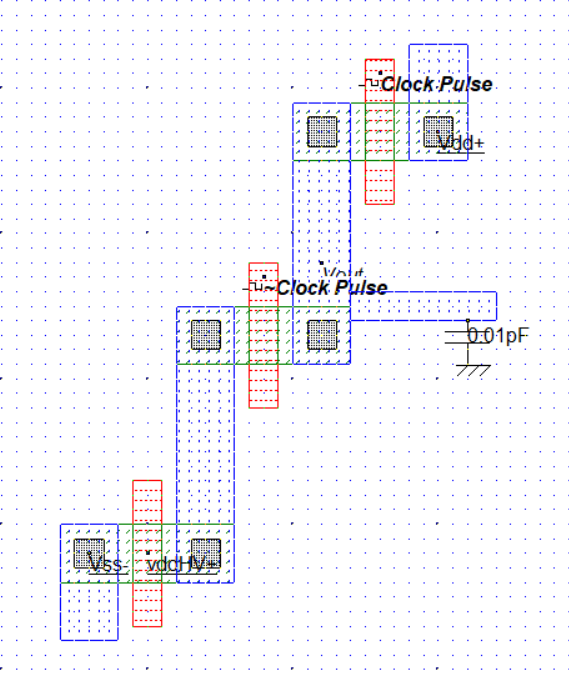
\includegraphics[width=0.6\textwidth]{ckt.png}
    \caption{Schematic of the NMOS ratio-less inverter circuit}
\end{figure}

\section*{Output}
\addcontentsline{toc}{section}{Output}

\begin{figure}[H]
    \centering
    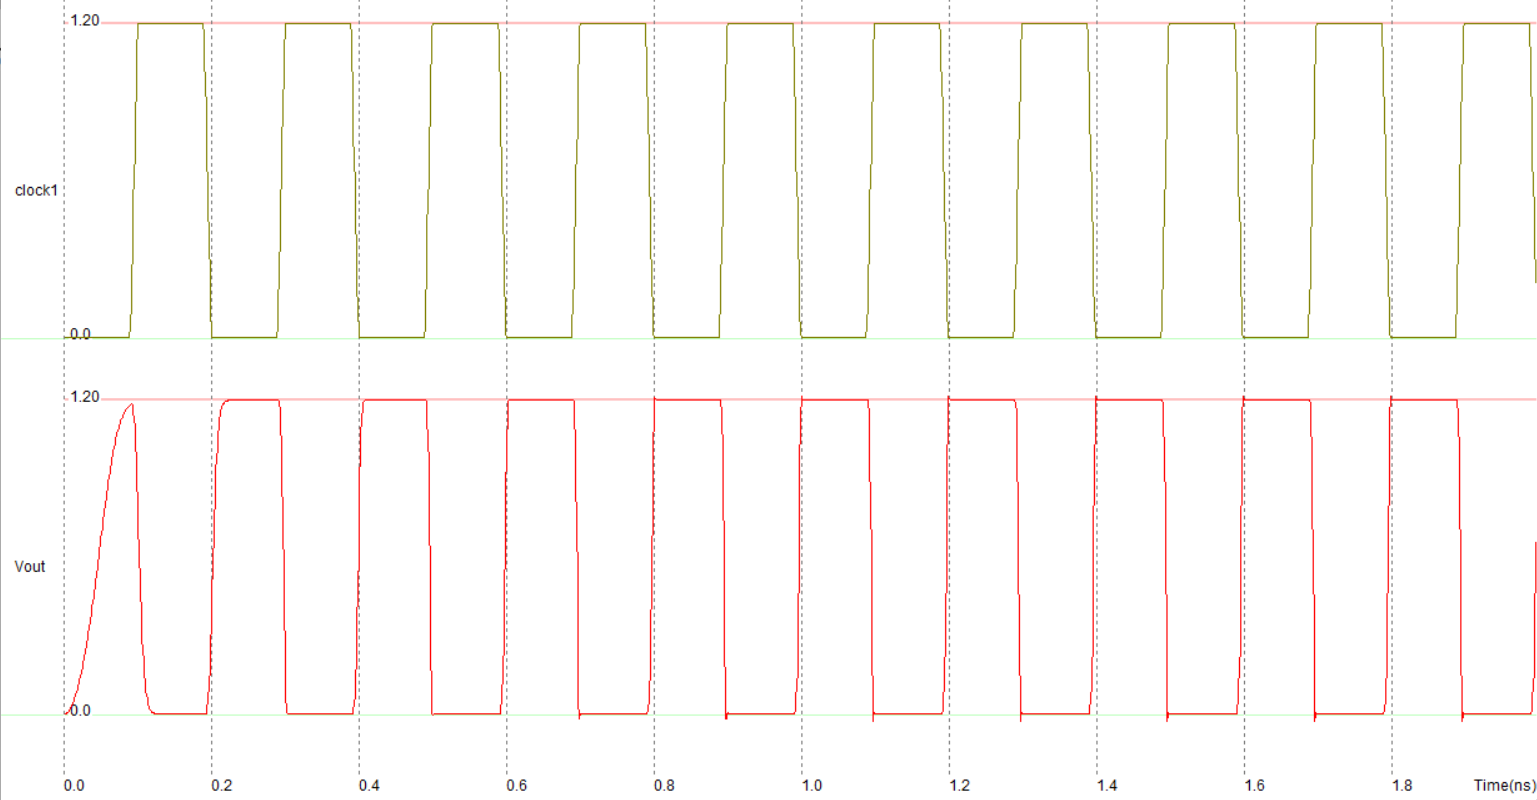
\includegraphics[width=0.75\textwidth]{11v_t.png}
    \caption{Plot of voltage over time without a capacitor.}
\end{figure}

\begin{figure}[H]
    \centering
    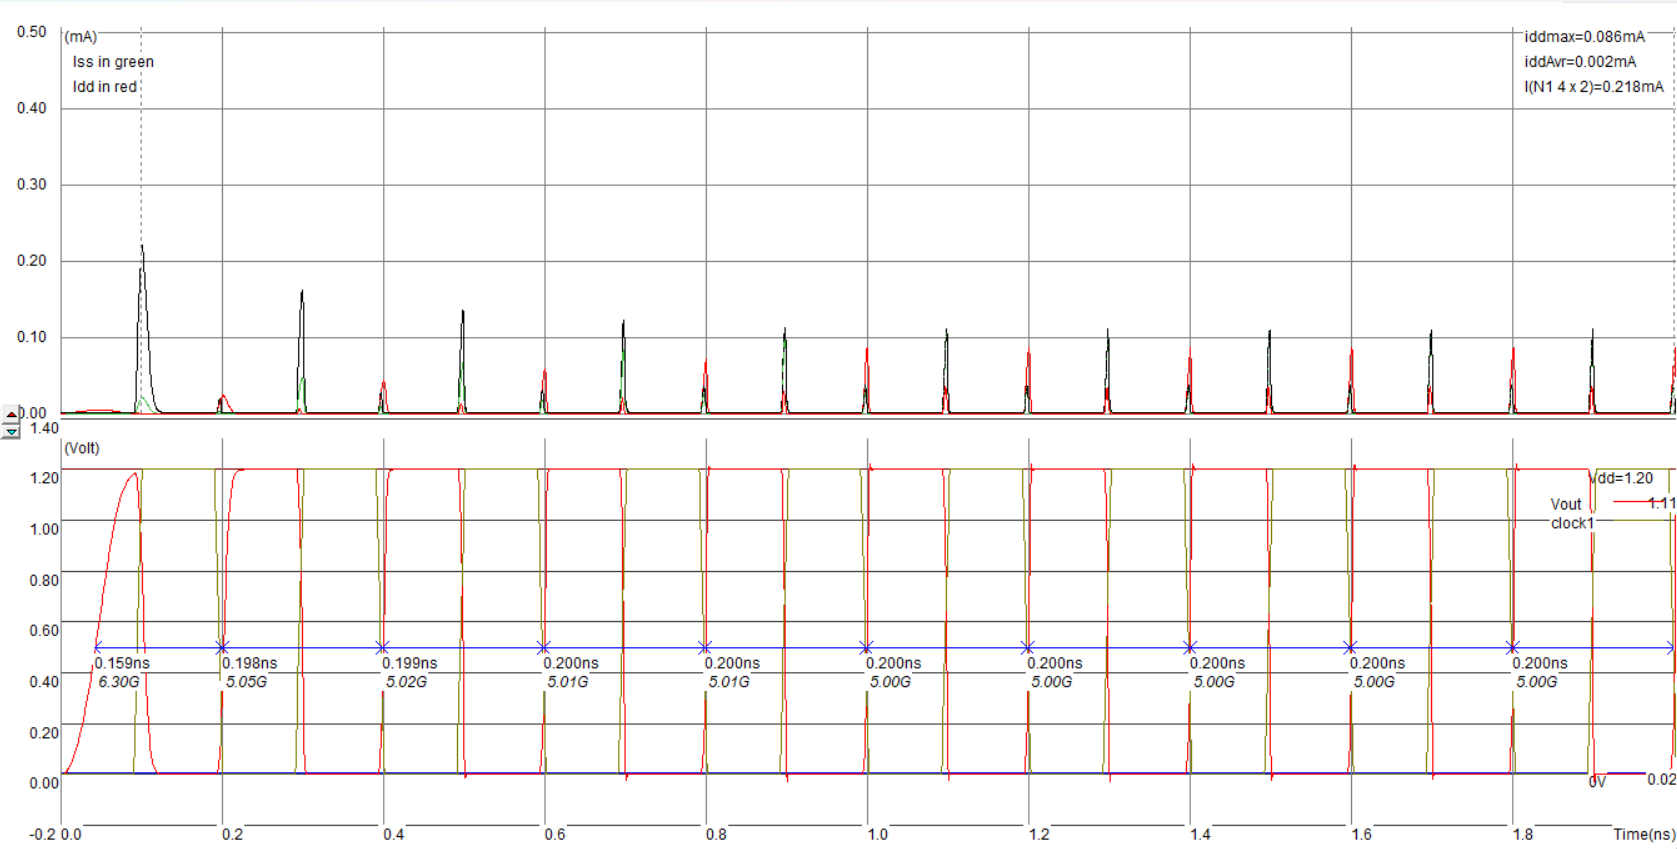
\includegraphics[width=0.75\textwidth]{21V_c.png}
    \caption{Plot of voltage versus current without a capacitor.}
\end{figure}

\begin{figure}[H]
    \centering
    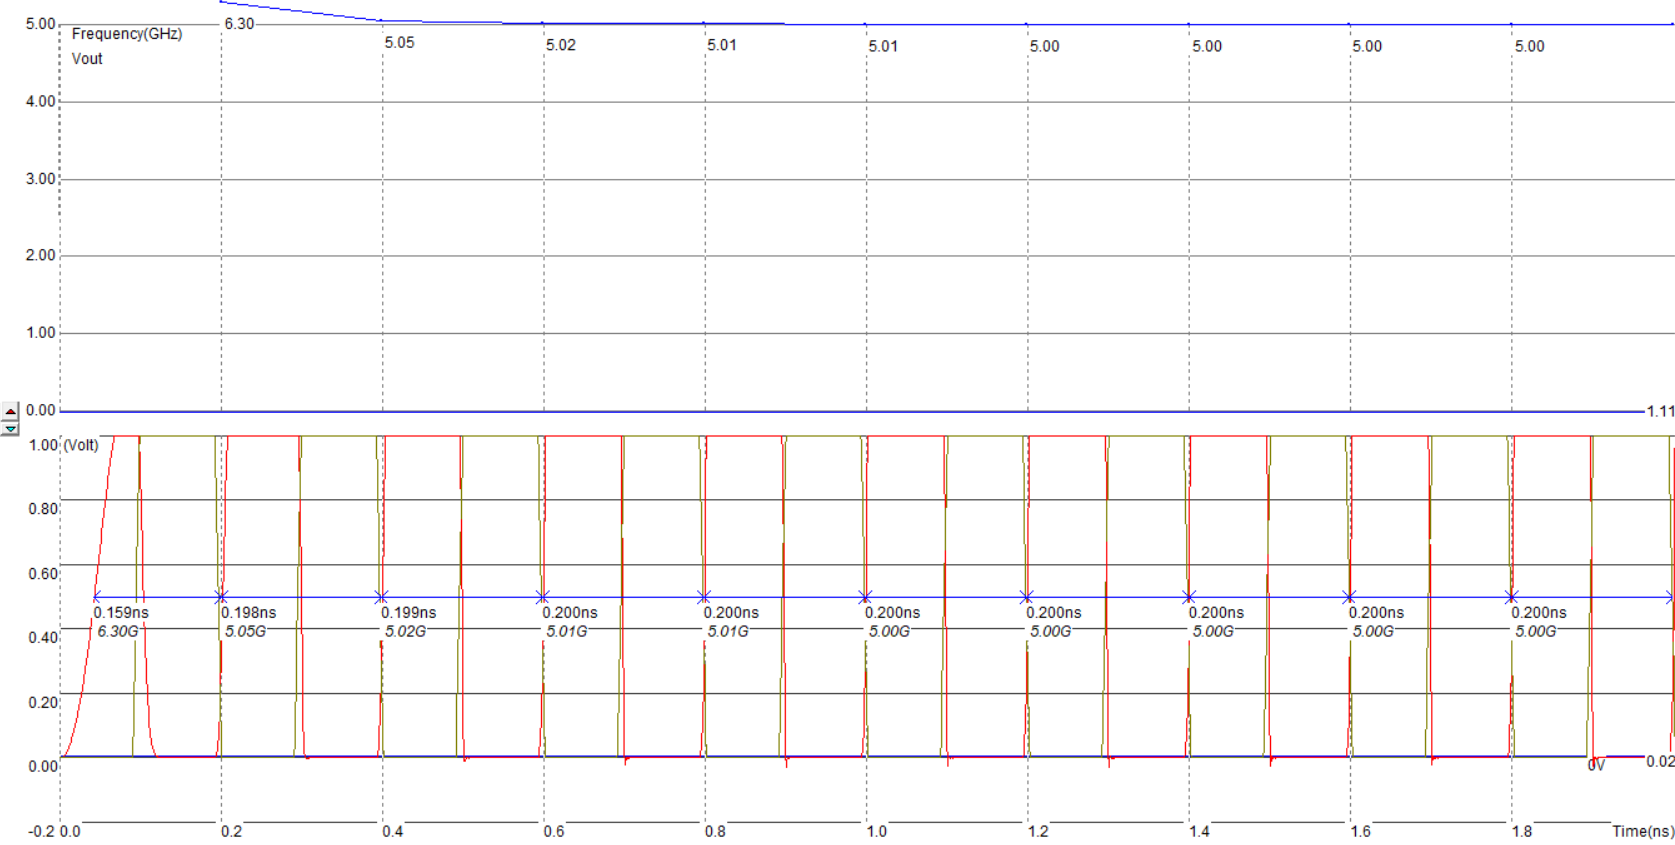
\includegraphics[width=0.75\textwidth]{31.png}
    \caption{Plot of frequency over time without a capacitor.}
\end{figure}

\begin{figure}[H]
    \centering
    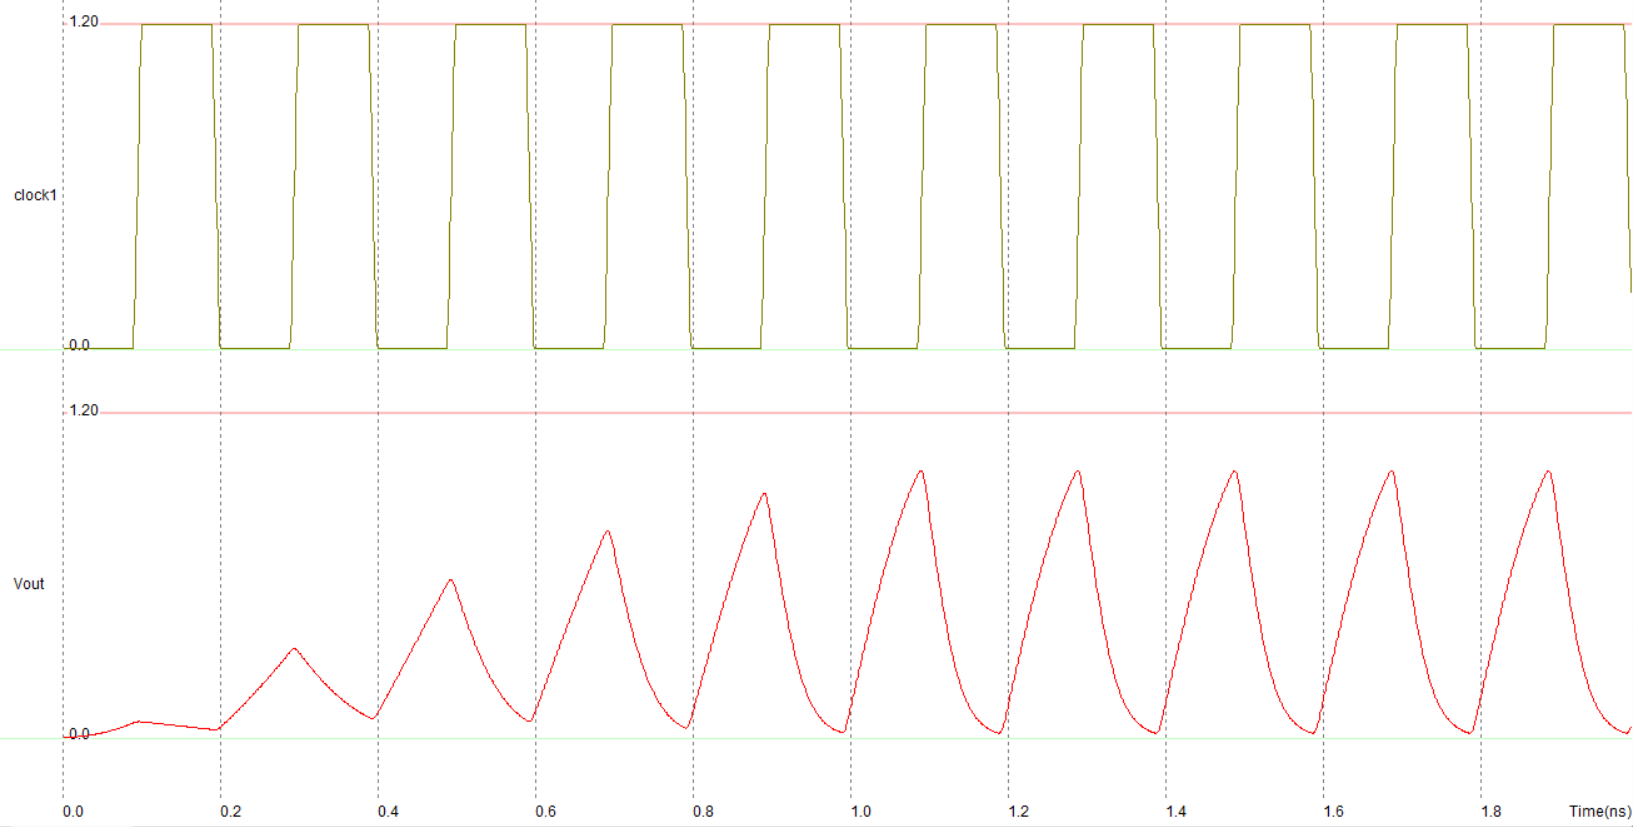
\includegraphics[width=0.75\textwidth]{41voltage_time.png}
    \caption{Plot of voltage over time with a capacitor.}
\end{figure}

\begin{figure}[H]
    \centering
    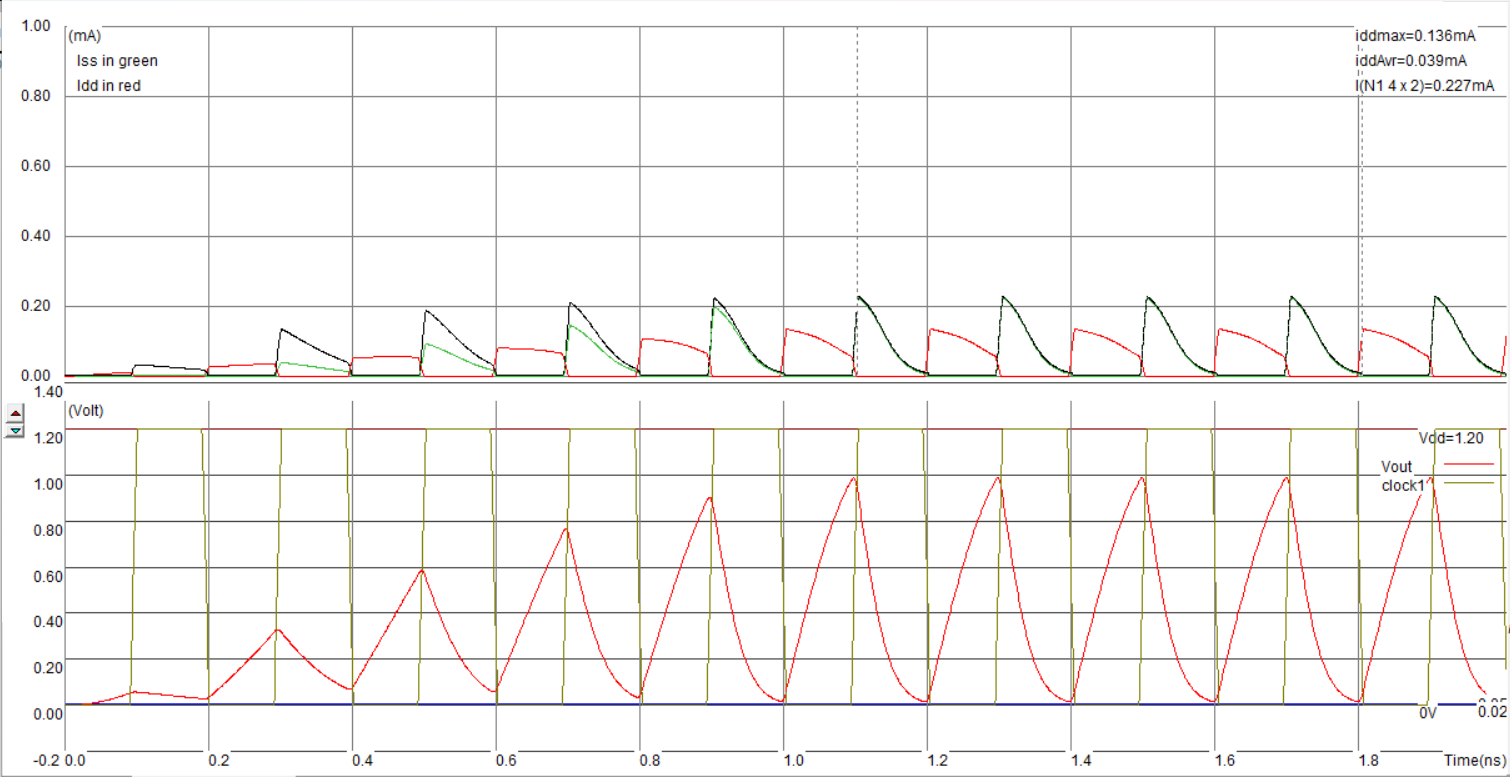
\includegraphics[width=0.75\textwidth]{51voltage_current.png}
    \caption{Plot of voltage versus current with a capacitor.}
\end{figure}

\begin{figure}[H]
    \centering
    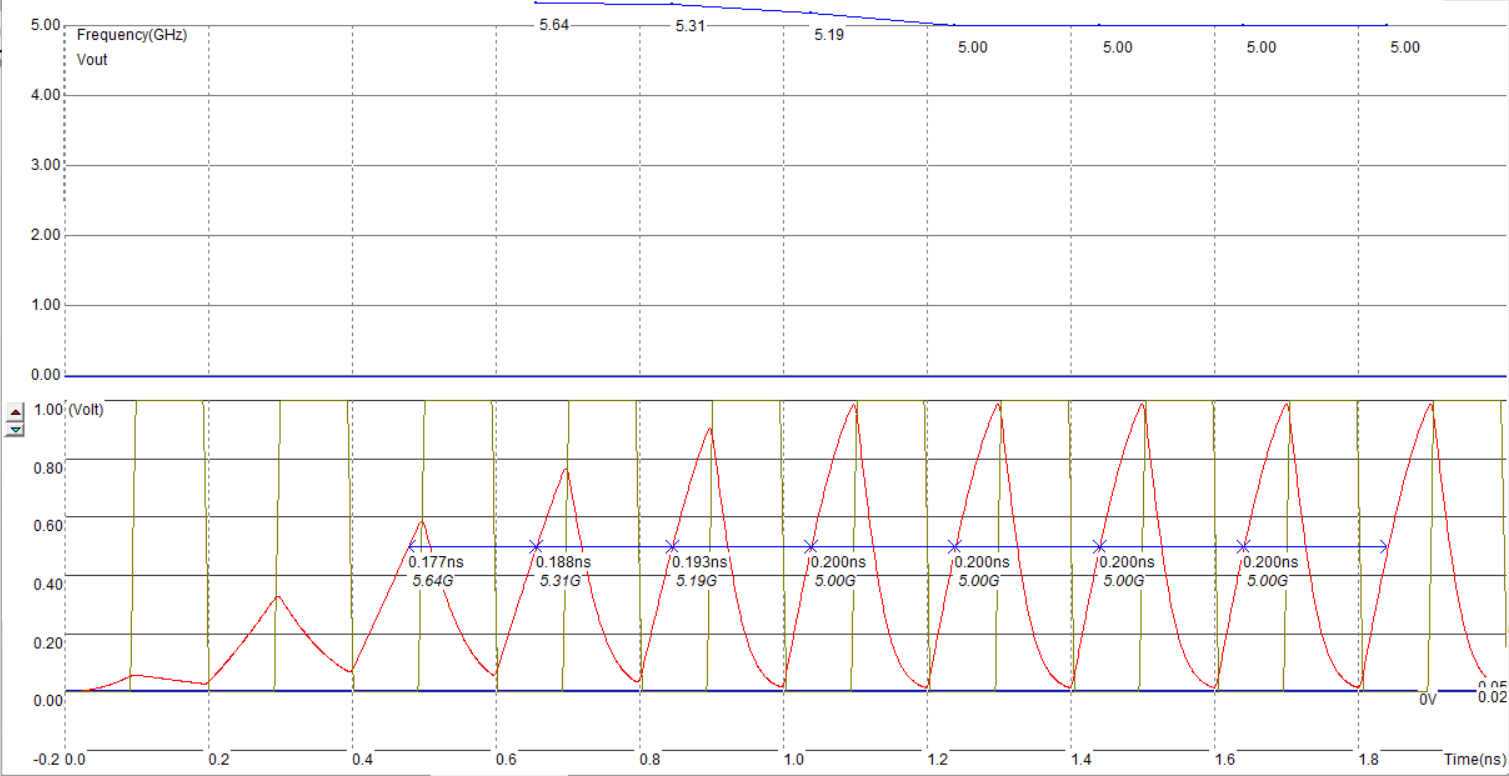
\includegraphics[width=0.75\textwidth]{61freq_time.png}
    \caption{Plot of frequency over time with a capacitor.}
\end{figure}

\section*{Discussion and Conclusion}
\addcontentsline{toc}{section}{Discussion and Conclusion}
In this experiment, a 3-NMOS ratio-less inverter was designed and simulated to analyze its switching characteristics and overall performance. The circuit consisted of one NMOS driver transistor and two NMOS active load transistors, removing the need for resistors. Simulations verified that the output was the logical inverse of the input: when the input was low, the active loads pulled the output high; when the input was high, the driver transistor pulled the output low.

The results indicated that the rise time was slower than the fall time, attributed to the weaker pull-up capability of the active loads. Additionally, static power dissipation was observed during the low output state due to continuous current flow. These outcomes are consistent with theoretical expectations, demonstrating how transistor biasing and active load design influence switching speed, delay, and power consumption.

A key observation was that the inverter’s switching threshold did not depend on transistor sizing ratios, which is a defining feature of ratio-less designs. Eliminating resistors makes the design more compatible with NMOS IC fabrication. Overall, this study reinforced important concepts in transistor operation, active loading, and the trade-offs between speed, power, and simplicity, providing valuable insights for VLSI design.
\bibliographystyle{IEEEtran}
\renewcommand{\bibname}{References}
\addcontentsline{toc}{section}{References}
\bibliography{ref}

\end{document}
